\documentclass[a4paper,12pt]{scrreprt}
    %% Used for changing geometry of the page
    %% Cover page text cannot overlay cover sketching/style 
    %% https://ctan.org/pkg/geometry?lang=en
\usepackage{geometry}
    %% Changes language of some packages protocols
    %% e.g., when captioning images: Figure 1. -> Figura 1.
    %% https://ctan.org/pkg/babel?lang=en
\usepackage[portuguese]{babel}
    %% Used for special fonts
    %% Cannot be compiled with pdflatex
    %% https://ctan.org/pkg/fontspec?lang=en
\usepackage{fontspec}
    %% Arial FONT
    \setmainfont{Arial}

    %% More colors and color options
    %% https://ctan.org/pkg/xcolor?lang=en
    %% https://ctan.org/pkg/colortbl?lang=en
\usepackage{xcolor,colortbl}
    %% More tabular options, like dashed/dotted lines
    %% https://ctan.org/pkg/arydshln?lang=en
\usepackage{arydshln}
    %% List of acronyms
    %% https://ctan.org/pkg/nomencl?lang=en
\usepackage[intoc]{nomencl}
    %% Must be called to init nomencl environment  
    \makenomenclature
    %% More images options/settings
    %% https://ctan.org/pkg/graphicx?lang=en
\usepackage{graphics}
    %% Defining subdirectories to image path enviornment
    %% \graphicspath{{sub1}{sub2}...{subN}}
    \graphicspath{{images}}
    
    %% used to handle cross-referencing commands in LaTeX to produce hypertext links in the document
    %% https://ctan.org/pkg/hyperref?lang=en
\usepackage{hyperref}
    %% math environments
    %% https://ctan.org/pkg/amsmath?lang=en

    %% settings
    \hypersetup{
        colorlinks,
        citecolor=black,
        filecolor=black,
        linkcolor=black,
        urlcolor=black
    }

\usepackage{amsmath}
    %% Defining backgrouns, used to make the cover
    %% https://ctan.org/pkg/background?lang=en
\usepackage[some]{background}
    %% Used to make drawings or complex graphics
    %% http://pgf.sourceforge.net/pgf_CVS.pdf
\usepackage{tikz}
    %% Tikz library to point operations ((x1,y1) + (x2,y2))
    \usetikzlibrary{calc}

\usepackage[most]{tcolorbox}
\tcbuselibrary{listings}
\usepackage{listings}
\usepackage{xcolor}

%% Defining sfdefault font and default font for document
\renewcommand{\familydefault}{\sfdefault}


%% Costume made cover 
%% From there you can use \makecover command to build the cover
\include{cover}

%==========================================================================
% DOCUMENT
%==========================================================================

\begin{document}

\pagenumbering{gobble}

% builds the cover
\makecover

%% smaller footer and header size
\newgeometry{top=3cm,left=3cm,right=3cm,bottom=4cm}

%==========================================================================
% BEGIN OPCIONAL DEDICATÓRIA
%==========================================================================

\clearpage
\begin{center}
    \thispagestyle{empty}
    \vspace*{\fill}
    
    $<<$/opcional Dedicatória$>>$
    
    \vspace*{\fill}
\end{center}
\clearpage

%==========================================================================
% END OPCIONAL DEDICATÓRIA
%==========================================================================


%==========================================================================
% BEGIN ABSTRACT PAGE
%==========================================================================



%% Abstract name: \Large font size, flushed left and paragraph skip before abstract content
\renewenvironment{abstract}
 {\par\noindent\textbf{\Large\abstractname}\par\bigskip}
 {}

\begin{flushleft}
\begin{abstract}
    <<O resumo tem como objectivo descrever de forma sucinta o trabalho realizado. Deverá conter uma pequena introdução, seguida por uma breve descrição do trabalho realizado e terminando com uma indicação sumária do seu estado final. Não deverá exceder as 400 palavras.>> 
    \par \textbf{Área de Aplicação}: <<Identificação da Área de trabalho. Por exemplo: Desenho e arquitectura de Sistemas de Bases de Dados.>> 
    \par \textbf{Palavras-Chave}: <<Conjunto de palavras-chave que permitirão referenciar domínios de conhecimento, tecnologias, estratégias, etc., directa ou indirectamente referidos no relatório. Por exemplo: Bases de Dados Relacionais, Gestão de Índices, JAVA, Protocolos de Comunicação.>>
\end{abstract}
\end{flushleft}


\pagebreak

%==========================================================================
% END ABSTRACT PAGE 
%==========================================================================

%==========================================================================
% BEGIN INDEXES PAGES
%==========================================================================

%% Changes table of content name
%% Portuguese babel default : "Conteúdo"
%% Personally I prefer "índice"
\renewcommand{\contentsname}{Índice}

\tableofcontents

\pagebreak

\listoffigures

\pagebreak

\listoftables

\pagebreak

%==========================================================================
% END INDEXES PAGES 
%==========================================================================


%==========================================================================
% BEGIN INTRODUCTION
%==========================================================================

%% Starting page numbering here
\pagenumbering{arabic}

\chapter{Introdução}
    <<Este primeiro capítulo deverá ter obrigatoriamente as subsecções abaixo apresentadas.>>
    \section{Contextualização}
        <<Nesta secção deverá ser apresentado o contexto no qual se desenvolve o caso de estudo seleccionado.>>
    \section{Apresentação do Caso de Estudo}
        <<Esta secção acolherá uma descrição concisa do caso de estudo seleccionado.>>
    \section{Motivação e Objectivos}
        <<Esta secção acolherá os diversos motivos, acompanhados por uma breve descrição, que conduziram à proposta e ao desenvolvimento do trabalho, assim como a apresentação detalhada dos diversos objectivos a alcançar com a sua realização.>>
    \section{Estrutura do Relatório}
        <<Após a leitura da introdução de um relatório é "simpático" apresentar uma breve descrição daquilo que se vai encontrar nos demais capítulos do relatório.>>

%==========================================================================
% END INTRODUCTION
%==========================================================================


%==========================================================================
% BEGIN SUGESTÕES PARA ESCRITA DO RELATÓRIO
%==========================================================================

\chapter{Sugestões para Escrita do Relatório}

    \section{Sugestões Gerais}
        <<O presente documento deverá servir de base para a escrita do relatório do trabalho realizado.>>\\

        <<O tipo de letra a utilizar deverá ser Arial.. Porém recomenda-se em situações de escrita de excertos de programas a utilização do tipo de letra Courier New.>>\\

        << Alguns estilos documento: Heading1, Heading2, Heading3, Normal e Footnote Text; foram especialmente modificados para os relatórios da presente disciplina.>>\\

        <<Os formatos e estilos de letra não devem estar constantemente a ser modificados ao longo do relatório. Tal situação dará origem a um relatório com um formato e apresentação muito heterogénea e com um aspecto pouco consistente.>>
    \section{Termos Estrangeiros}
        <<Os termos estrangeiros utilizados deverão ser apresentados num formato diferente do resto do texto, por exemplo: Data Warehouse (em itálico) ou "Data Warehouses" (entre aspas), devendo ser evitados sempre que se conheça uma tradução correcta para português. Para validação desses termos existem vários dicionários no mercado que poderão ser úteis.>>
    \section{Tabelas e Figuras}
        <<Caso seja necessário introduzir figuras ou tabelas no corpo do documento, estas devem seguir os formatos que se apresentam de seguida. Qualquer figura ou tabela deverá ter uma legenda associada, devendo esta estar correctamente apresentada no índice respectivo no início do relatório.>>
        

         \begin{figure}[!h]
            \centering
            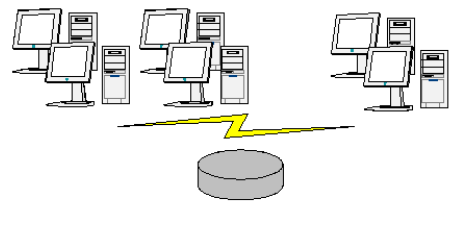
\includegraphics[scale=0.7]{images/example.png}
            \caption{Ilustração de inserção de uma figura e legenda.}
         \end{figure}
        
        \vspace*{0.2cm}
        
        \begin{table}[!h]
            \centering
            \begin{tabular}{|p{2cm}|p{2cm}|p{2cm}|p{2cm}|p{2cm}|}
               \hline
               \rowcolor{gray!20!white}
                Coluna1 & Coluna2 & Coluna3 & & ColunaN \\
                \hline
                        &         &         & &         \\
                \hline
                        &         &         & &         \\
                \hline
                        &         &         & &         \\
                \hline
                        &         &         & &         \\
                \hline
                        &         &         & &         \\
                \hline
            \end{tabular}
            \caption{Ilustração de inserção de uma tabela e sua legenda.}
        \end{table}
        
        
    \section{Siglas e Acrónimos}
        <<A utilização de siglas ou acrónimos deverão, tal como os termos estrangeiros, ser feita com base no seguinte formato: Bases de Dados (BD). Todas as siglas e acrónimos deverão ser apresentadas numa secção própria, no início (a seguir aos índices) ou no final (a seguir ao capítulo das conclusões e trabalho futuro) do relatório.
    \section{Referências Bibliográficas}
        <<A forma de apresentação das referências bibliográficas deverão estar de acordo com as regras definidas pela IEEE. Consultar www.ieee.org>>
    \section{Tipo de Ficheiro}
        <<O relatório poderá ser enviado para o regente da disciplina por correio electrónico num dos seguintes formatos: html, word ou pdf>>
   
        
%==========================================================================
% END SUGESTÕES PARA ESCRITA DO RELATÓRIO
%==========================================================================


\chapter{Conceção e Engenharia de Requisitos Assistida por LLM}
<<Nesta etapa pretende-se definir claramente o problema e o domínio de aplicação do sistema, introduzir os LLM como agentes de apoio cognitivo ao processo de Engenharia de Requisitos e produzir a documentação formal de requisitos necessária, de forma estruturada e alinhada com as normas reconhecidas, para servir como base as etapas seguintes do projeto.>>

\section{Definição do domínio do sistema}

\subsection{Contextualização}

A empresa EcoRide Solutions é uma oficina de média dimensão situada em Braga, especializada na reparação e manutenção de trotinetes elétricas. Fundada em 2018 por João Martins, antigo técnico de eletrónica, e Ana Ribeiro, gestora com experiência na área da mobilidade urbana, a empresa cresceu rapidamente devido ao aumento da utilização de trotinetes como meio de transporte alternativo. Atualmente, a oficina conta com uma equipa de oito colaboradores, incluindo técnicos especializados, um responsável de armazém e uma assistente administrativa.

Com o aumento do volume de trabalho, a gestão manual dos processos começou a revelar-se insuficiente. A empresa lida diariamente com dezenas de pedidos de diagnóstico, reparações complexas, encomendas de peças e emissão de faturas. A ausência de um sistema integrado tem originado atrasos, falhas de comunicação interna e dificuldades no controlo de custos e de stock. A gerência reconhece que, para manter a competitividade e garantir a qualidade do serviço, é necessário modernizar os processos operacionais.

\subsection{Fundamentação}

A necessidade de implementar um sistema informático surge da crescente complexidade das operações da oficina. Os processos atuais, baseados em folhas de cálculo, documentos dispersos e registos manuais, dificultam a rastreabilidade das intervenções e comprometem a fiabilidade da informação. A inexistência de um mecanismo centralizado para gerir clientes, equipamentos, ordens de serviço e peças conduz a erros frequentes, como discrepâncias no stock, perda de histórico técnico e dificuldades na elaboração de relatórios financeiros.

Além disso, a expansão do mercado de micromobilidade exige que a empresa adote ferramentas que permitam maior eficiência operacional e capacidade de resposta. A automatização dos processos administrativos e técnicos permitirá reduzir tempos de execução, melhorar a comunicação entre técnicos e administração e aumentar a transparência perante o cliente. A implementação de um sistema de gestão integrado constitui, assim, um passo estratégico para a sustentabilidade e crescimento da empresa.

\subsection{Objetivos}

O \textbf{objetivo geral} é desenvolver um sistema de gestão integrado que suporte e otimize os processos operacionais, técnicos e administrativos de uma oficina de reparação de trotinetes.

Os \textbf{objetivos específicos} são:
\begin{itemize}
	\item Garantir o registo estruturado de clientes, equipamentos e histórico de intervenções;
	\item Controlar o ciclo completo das ordens de serviço, desde o diagnóstico até à entrega;
	\item Registar tempos de reparação, peças utilizadas e custos associados;
	\item Automatizar a gestão de stock, incluindo entradas, saídas e alertas de reposição;
	\item Integrar a faturação de serviços e peças, assegurando conformidade legal;
	\item Disponibilizar relatórios técnicos e financeiros para apoio à decisão;
	\item Melhorar a comunicação interna e reduzir erros operacionais.
\end{itemize}


\subsection{Viabilidade}

A implementação do sistema apresenta viabilidade económica e operacional. Estima-se que o desenvolvimento e implementação tenham um custo inicial entre \textbf{12 000 € e 18 000 €}, dependendo da complexidade dos módulos e da necessidade de integrações externas. Os custos anuais de manutenção e suporte poderão situar-se entre \textbf{1 000 € e 2 500 €}.

Com base nos dados da empresa, calcula-se que a automatização dos processos permita reduzir o tempo administrativo em cerca de \textbf{30\%}, o que representa uma poupança anual aproximada de \textbf{6 000 €} em horas de trabalho. A melhoria no controlo de stock poderá reduzir perdas e compras desnecessárias, estimando-se um ganho adicional de \textbf{2 000 € a 3 000 €} por ano. A redução de erros de faturação e a melhoria na gestão das ordens de serviço poderão ainda aumentar a receita anual em cerca de \textbf{5\%}, o que, para um volume médio de faturação de \textbf{150 000 €}, representa \textbf{7 500 €}.

Assim, o retorno do investimento poderá ser alcançado entre \textbf{12 e 18 meses}, demonstrando a viabilidade económica do projeto.

\subsection{Delimitação do Domínio}

O domínio do sistema abrange todos os processos relacionados com a gestão operacional de uma oficina de reparação de trotinetes, incluindo:
\begin{itemize}
	\item Gestão de entidades (clientes, trotinetes, técnicos);
	\item Gestão de ordens de serviço e respetivos estados;
	\item Processos de diagnóstico e reparação;
	\item Gestão de peças, consumíveis e stock;
	\item Processos de faturação e emissão de documentos;
	\item Geração de relatórios operacionais e financeiros;
\end{itemize}

Não estão incluídos no domínio:
\begin{itemize}
	\item Gestão de recursos humanos;
	\item Integração com plataformas externas de mobilidade (exceto se definido como requisito futuro);
	\item Funcionalidades de e-commerce ou portal de cliente (fora do escopo inicial).
\end{itemize}


\subsection{Recursos}

\subsection{Equipa de Trabalho}

\subsection{Plano de Execução}


\section{Identificação de stakeholders}

\subsection{Stakeholders Internos}

<<Breve descrição do que são "stakeholders internos".>>

\begin{tcolorbox}[
	title={Gerência: João Martins e Ana Ribeiro},
	colback=white,
	colframe=black,
	arc=2mm,
	boxrule=0.5pt
	]
	\textbf{Papel:} Responsáveis pela direção estratégica da EcoRide Solutions. \par
	\textbf{Interesse:} Obter visibilidade total sobre o desempenho operacional, financeiro e técnico da oficina. \par
	\textbf{Influência:} Elevada; têm poder de decisão sobre requisitos, prioridades e investimentos. \par
	\textbf{Necessidades principais:} Relatórios financeiros e técnicos, indicadores de desempenho, controlo de custos, rastreabilidade das operações. \par
	\textbf{Interação com o sistema:} Consulta de dashboards, relatórios e validação de decisões operacionais.
\end{tcolorbox}

\begin{tcolorbox}[
	title={Assistente Administrativa},
	colback=white,
	colframe=black,
	arc=2mm,
	boxrule=0.5pt
	]
	\textbf{Papel:} Responsável pelo atendimento ao cliente, criação de ordens de serviço, faturação e arquivo documental. \par
	\textbf{Interesse:} Simplificação das tarefas administrativas e redução de erros. \par
	\textbf{Influência:} Moderada; utiliza o sistema diariamente e fornece feedback operacional. \par
	\textbf{Necessidades principais:} Registo rápido de clientes e equipamentos, emissão de faturas, gestão de documentos e comunicação com clientes. \par
	\textbf{Interação com o sistema:} Inserção e atualização de dados, emissão de documentos, consulta de histórico.
\end{tcolorbox}

\begin{tcolorbox}[
	title={Técnicos de Reparação},
	colback=white,
	colframe=black,
	arc=2mm,
	boxrule=0.5pt
	]
	\textbf{Papel:} Executam diagnósticos, intervenções e reparações nas trotinetes. \par
	\textbf{Interesse:} Acesso rápido ao histórico técnico e registo eficiente das intervenções. \par
	\textbf{Influência:} Moderada; impactam diretamente a qualidade dos dados técnicos. \par
	\textbf{Necessidades principais:} Registo de diagnósticos, tempos de reparação, peças utilizadas e estados das ordens de serviço. \par
	\textbf{Interação com o sistema:} Atualização de ordens de serviço, consulta de instruções e histórico de reparações.
\end{tcolorbox}

\begin{tcolorbox}[
	title={Responsável de Armazém},
	colback=white,
	colframe=black,
	arc=2mm,
	boxrule=0.5pt
	]
	\textbf{Papel:} Gere o stock de peças, consumíveis e materiais. \par
	\textbf{Interesse:} Manter níveis de stock adequados e evitar ruturas ou excesso de inventário. \par
	\textbf{Influência:} Moderada; contribui para a definição de regras de stock e reposição.\par
	\textbf{Necessidades principais:} Registo de entradas e saídas, alertas de stock mínimo, integração com ordens de serviço. \par
	\textbf{Interação com o sistema:} Atualização de inventário, consulta de necessidades de peças, validação de consumos.
\end{tcolorbox}


\subsection{Stakeholders Externos}

<<Breve descrição do que são "stakeholders externos".>>

\begin{tcolorbox}[
	title={Clientes da Oficina},
	colback=white,
	colframe=black,
	arc=2mm,
	boxrule=0.5pt
	]
	\textbf{Papel:} Proprietários das trotinetes que recorrem aos serviços da empresa. \par
	\textbf{Interesse:} Transparência no processo de reparação, prazos cumpridos e custos claros. \par
	\textbf{Influência:} Baixa; não intervêm no desenvolvimento, mas influenciam requisitos de qualidade. \par
	\textbf{Necessidades principais:} Informação sobre o estado da reparação, histórico de serviços, faturas e orçamentos. \par
	\textbf{Interação com o sistema:} Indireta; através de documentos emitidos e comunicação da oficina.
\end{tcolorbox}

\begin{tcolorbox}[
	title={Fornecedores de Peças},
	colback=white,
	colframe=black,
	arc=2mm,
	boxrule=0.5pt
	]
	\textbf{Papel:} Entidades que fornecem componentes e consumíveis. \par
	\textbf{Interesse:} Processos de encomenda claros e previsíveis. \par
	\textbf{Influência:} Baixa; apenas afetam o módulo de stock e compras. \par
	\textbf{Necessidades principais:} Informação sobre necessidades de reposição e histórico de compras. \par
	\textbf{Interação com o sistema:} Indireta; através de registos de encomendas e receção de material.
\end{tcolorbox}


\subsection{Stakeholders Técnicos}

<<Breve descrição do que são "stakeholders técnicos".>>

\begin{tcolorbox}[
	title={Equipa de Desenvolvimento do Sistema},
	colback=white,
	colframe=black,
	arc=2mm,
	boxrule=0.5pt
	]
	\textbf{Papel:} Responsáveis pela análise, implementação e manutenção do software. \par
	\textbf{Interesse:} Requisitos claros, estabilidade do sistema e facilidade de manutenção. \par
	\textbf{Influência:} Elevada; definem a arquitetura e viabilidade técnica. \par
	\textbf{Necessidades principais:} Especificações completas, acesso a utilizadores-chave, feedback contínuo. \par
	\textbf{Interação com o sistema:} Desenvolvimento, testes, manutenção e evolução.
\end{tcolorbox}

\section{LLM e Avaliação}

\textbf{Objetivo:} Apresentar tema e do sistema a definir

\begin{tcolorbox}[
	listing only,
	breakable,
	enhanced,
	colback=white,
	colframe=black,
	listing options={
		breaklines=true,
		basicstyle=\ttfamily\small
	}
	]
	Considera o seguinte tema para a implementação de um sistema informático (Efetua apenas uma análise breve, não inicies nenhum processo criativo): <<Tema 3 no enunciado do trabalho prático>>
\end{tcolorbox}

\textbf{Análise Crítica:} Avaliar resultados...

\textbf{Objetivo:} Definir o contexto do problema e objetivos a atingir
\begin{tcolorbox}[
	listing only,
	breakable,
	enhanced,
	colback=white,
	colframe=black,
	listing options={
		breaklines=true,
		basicstyle=\ttfamily\small
	}
	]
	Age como um engenheiro de requisitos. Define o dominio do sistema para o tema apresentado. Apresenta os seguintes tópicos: \\
	- Contextualização (2 a 3 parágrafos): apresenta o contexto e uma história para uma potencial empresa com pessoas reais; \\
	- Fundamentação (2 a 3 parágrafos): apresenta a causa/s para a implementação do sistema \\
	- Objetivos a atingir \\
	- Viabilidade: simula potenciais valores \\
	Podes apresentar mais tópicos que aches necessários, mas o foco deverão ser os apresentados. Utiliza uma linguagem técnica e formal, adequada para um relatório académico. Evita "bullet points" na contextualização e fundamentação.
\end{tcolorbox}

\textbf{Análise Crítica:} Avaliar resultados...

\textbf{Objetivo:} Definir os stakeholders de forma estruturada
\begin{tcolorbox}[
	listing only,
	breakable,
	enhanced,
	colback=white,
	colframe=black,
	listing options={
		breaklines=true,
		basicstyle=\ttfamily\small
	}
	]
	A próxima tarefa é identificar os stakeholders, sendo coerente com a definição do sistema gerada. Apresenta o nome de cada stakeholder (nos casos que se aplique), o seu papel, interesse, influência, necessidades principais (nos casos que se aplique) e o tipo de interação com o sistema. Agrupa os stakholders em grupos (e.g: pessoal interno e externo).
\end{tcolorbox}
\textbf{Análise Crítica:} Avaliar resultados...



%==========================================================================
% BEGIN CONCLUSÕES DE TRABALHO FUTURO
%==========================================================================

\chapter{Conclusões e Trabalho Futuro}
    <<Elaborar uma apreciação crítica sobre o trabalho realizado, apontando os seus pontos fortes e fracos. Adicionalmente, caso se aplique, enunciar eventuais tarefas a realizar futuramente ou novas opções para estender o trabalho realizado.>>


%==========================================================================
% END CONCLUSÕES DE TRABALHO FUTURO
%==========================================================================

%==========================================================================
% BEGIN REFERÊNCIAS
%==========================================================================

%% Changes biblibography name
%% Portuguese babel default : "Bibliografia"
%% Personally I prefer "Referências"
\renewcommand\bibname{Referências}

%% https://www.overleaf.com/learn/latex/bibliography_management_with_bibtex
\begin{thebibliography}{9}
<<Apresentar a lista de referências bibliográficas referidas ao longo do relatório; recomenda-se a utilização do formato Harvard - http://libweb.anglia.ac.uk/referencing/harvard.htm>>
\end{thebibliography}


%==========================================================================
% END REFERÊNCIAS
%==========================================================================

%==========================================================================
% BEGIN LISTA DE SIGLAS E ACRÓNIMOS
%==========================================================================

%% Portuguese babel does not translate this environment
\renewcommand{\nomname}{Lista de Siglas e Acrónimos}

%% Text that can be shown before acronyms list
\renewcommand{\nompreamble}{<<Apresentar uma lista com todas as siglas e acrónimos utilizados durante a realização do trabalho. O formato base para esta lista deverá ser da forma como abaixo se apresenta.>>}

%% acronyms
\nomenclature[01]{\textbf{BD}}{Base de Dados}
\nomenclature[02]{DW}{Data Warehouse}
\nomenclature[03]{OLTP}{On-Line Analytical Processing}
\nomenclature[04]{...}{...}

%% Show acronyms
\printnomenclature



%==========================================================================
% END LISTA DE SIGLAS E ACRÓNIMOS
%==========================================================================


%==========================================================================
% BEGIN ANEXOS
%==========================================================================

%% Why \addchap, instead of \chapter? 
%% \addchap has no numbering but appears in table of contents.
\addchap{Anexos}

    <<Os anexos deverão ser utilizados para a inclusão de informação adicional necessária para uma melhor compreensão do relatório o para complementar tópicos, secções ou assuntos abordados. Os anexos criados deverão ser numerados e possuir uma designação. Estes dados permitirão complementar o Índice geral do relatório relativamente à enumeração e apresentação dos diversos anexos.>>
    
    %% section version of \addchap
    \addsec{Anexo 1}


%==========================================================================
% END ANEXOS
%==========================================================================
\end{document}